%\documentclass{minimal}
\documentclass{article}
\usepackage[utf8]{inputenc}
\usepackage{amsmath}
\usepackage{amssymb}
\usepackage{multicol}
\usepackage{tikz}
\usetikzlibrary{arrows}
\tikzstyle{level 1}=[sibling distance=4cm]
\tikzstyle{level 2}=[sibling distance=1.5cm]
\tikzstyle{level 3}=[sibling distance=.5cm]
\title{Osztott rendszerek szintézise\\1. tétel}
\begin{document}
%\maketitle
\section*{Feladatok specifikációja, étkező filozófusok, absztrakt program fogalma, szemantikája}
Adott 5 filozófus [együttműködő párhuzamos folyamatok] és egy tál étel [közös erőforrás]. A filozófusok körben ülnek, minden két filozófus között egy-egy villa. A filozófus csak akkor tud enni, ha mind a két keze ügyében levő villát birtokba veszi, de csak akkor tudja a villákat megfogni, ha azok éppen szabadok. Ebből következik, hogy szomszédos filozófusok nem tudnak egyidejűleg enni. A két villát (a két villát egyszerre, de csak ha szabad!) felvehetik, lerakhatják, ehetnek és (végül) hazamehetnek. Ezeket a tevékenységeket állapotok fogják a specifikációban jelezni.
\\\\
Legyen az 5 filozófus: $f_0,..,f_4$\\\\
Legyen az $i.$ filozófus állapota
\begin{multicols}{2}
\begin{enumerate}
\item[$f_g$]– ha gondolkodik,
\item[$f_v$]– ha kezében van a két villa,
\item[$f_e$]– ha eszik és
\item[$f_o$]– ha otthon van.
\end{enumerate}
\end{multicols}
A következőkben a 7 féle specifikációs feltétel segítségével formálisan is specifikáljuk a fenti feladatot. Fontos látni, hogy a párhuzamos programok specifikációja nem a hagyományos előfeltétel-utófeltétel párossal fogalmazható meg, hiszen itt a szó hagyományos értelmében sose áll majd meg a program, tehát nincs is értelme utófeltételről beszélni. Ugyanakkor a programok végső soron itt is állapotátmenetek sorozatait produkálják, ezért az előfeltétel mellett az állapotok közti kapcsolatok, átmenetek jellemzésével tudjuk a feladatspecifikációt elvégezni.
\\
\\
(Ahol i. filozófus szerepel, ott mindig úgy kell érteni, hogy külön áll a kikötés minden i-re ahol $i \in [0..4]$)
\\\\
Az első kikötés, hogy minden filozófusra igaz, hogy ha most gondolkodik éppen, akkor vagy örökké ebben az állapotban fog maradni, vagy kezébe veszi a villákat vagy hazamegy. Tehát olyan biztosan nem fordulhat elő, hogy egy gondolkodó filozófus (villák nélkül) enni kezdjen. Az ilyen jellegű kikötéseket lehet az "amíg nem" alakú mondatokkal megadni. P és Q logikai függvényekre (azaz: $P:A \rightarrow \mathbb{L} $ )
kiolvasása: "addig marad igaz P, amíg nem igaz Q". Tehát P igazsághalmazát csak Q igazsághalmazán keresztül lehet közvetlenül elhagyni: "P és nem Q"-ból nem juthatunk egy lépésben "nem P"-be,
kivéve, ha "Q" igazzá válik. A másik lehetőség, amit szabad pedig, hogy "P" igaz marad. Az említett kikötés formálisan: $f_i.g \triangleright f_i.v \lor f_i.o$

Feltételezhetjük azt is, hogy ha egyszer egy filozófus megkaparintotta a villáit, akkor (hiszen mi másért szerezte meg) használni is fogja, mielőtt bármi mást tenne, tehát a "villák birtoklásának" állapotát csak az "evés" állapotán keresztül hagyhatjuk el: $f_i.v \triangleright f_i.e $

Ez a fajta kikötés egy stabilitási, illetve biztonságossági kikötés volt. Stabilitási mert arról szól, hogy "P" egészen addig stabilan igaz marad, amíg "Q" nem, és biztonságossági mert bizonyos állapotátmeneteket (jelesül ami "P és nem Q"-ból "nem P és nem Q"-ba vinne) tilt. Hogy ez miért a biztonságról szól, arra jó példa az ismert atomerőműs analógia, legyen P az, hogy "az atomerőmű biztonságosan üzemel", ekkor P tagadása az, hogy "felrobbant vagy legalábbis sansz van rá". Q pedig legyen az, hogy "szól az erőmű vészjelző szirénája". Nyilván azt szeretnénk, hogy vagy legyen végig biztonságos a
működés, vagy ha baj van, akkor időben értesüljünk erről. De semmiképpen ne történjen meg az, hogy minden rendben van (azaz P és nem Q), majd hirtelen minden figyelmeztetés nélkül megtörténik a baj (nem P és nem Q).

A modell kikötéseit úgy kell érteni, hogy a majdani megoldó programnak ezeknek a kikötéseknek mindig meg kell felelni, amikor a feltételeik teljesülnek. Azaz, ha egyszer P és nem Q-ban vagyok, majd Q-n keresztül elhagytam P-t, akkor bármikor, amikor a program futása visszajuttat P és nem Q-ba, akkor ugyanúgy teljesülnie kell a  $\triangleright$ -- "háromszög" tulajdonságnak.

Egy másik fajta kikötés, ha bizonyos állapotátmenet-változásokat kifejezetten el is várunk. Az "amíg nem" tulajdonság ugyan kikötötte, hogy P-t csak Q-n keresztül hagyhatjuk el, de azt már nem biztosította, hogy ez az átmenet valaha meg is fog történni. Őmiatta akár örökké maradhatunk "P és nem Q"-ban. A "biztosítja" kikötés annyival több az "amíg nem" tulajdonságnál, hogy itt valamikor meg kell történnie annak az átmenetnek, ami Q-t igazzá teszi. P-t nem feltétlenül kell elhagynunk, az a lényeg, hogy Q váljon igazzá. Persze, amint "P és Q"-ba jutottunk, nem teljesül a kikötés feltétele, tehát "P és Q"-ból már bármi történhet. Az ilyen jellegű kikötéseket összefoglalóan haladási tulajdonságoknak nevezzük. A következő sorban azt kötjük ki, hogy az evést előbb-utóbb biztosan fel kell váltania a gondolkodásnak. $f_i.e \mapsto f_i.g$

Szintén haladási feltétel, de kissé lazább kapcsolatot jelent az "elkerülhetetlen" tulajdonság. "P-ből elkerülhetetlenül bekövetkezik Q": garantáltan, ha most P igazsághalmazában vagyok, akkor előbb-utóbb eljutok Q igazsághalmazába. Arra azonban nincs semmilyen megkötés, hogy mikor és hogy közben milyen átmenetek történnek. Ez a feltétel azt fejezi ki, hogy minden filozófus, aki valamikor gondolkodni kezd, biztosan haza is fog jutni valaha: $f_i.g \hookrightarrow f_i.o$

Invariáns az, aminek a rendszer futásának minden pillanatában igaznak kell lennie, másképp megfogalmazva semmilyen értékadás nem vihet ki az invariáns tulajdonság igazsághalmazából. Itt invariáns az, hogy szomszédos filozófusok biztosan nem étkeznek egyszerre (Az összeadást és kivonást modulo 5 kell érteni).
$(f_i.e \rightarrow \neg f_{i\oplus1}.e \land f_{i\ominus1}.e) \in inv$

A fixpont-kikötések szólnak arról, minek kell teljesülnie, ha a program fixpontba jut. A fixpont az az állapot (több ilyen is lehet, de egyáltalán nem biztos, hogy van ilyen), ahol az egyébként végtelenül futó program gyakorlatilag leáll, mert hiába fut még tovább, garantáltan nem történik már állapotváltozás. Fontos, a következő kikötés NEM azt mondja meg, hogy mikor vagyunk fixpontban, hanem azt, hogy HA fixpontba jutottunk, akkor onnantól ennek az állításnak kell igaznak lennie. Azaz, ha a program megáll, akkor biztosan minden filozófus már otthon van. Másképp megfogalmazva, biztosan nem érhet véget a program érdemi működése addig, amíg nincs mindenki otthon. $fp \Rightarrow f_i.o$ Ha a program sose "áll le", akkor bármilyen FP-kikötésnek megfelel.

A következő fajta a kikötés a terminálási tulajdonság. Ezzel fejezzük ki, hogy egy bizonyos kezdőállapotból (nevezetesen, amikor minden filozófus gondolkodik), garantáltan el kell érnünk a fixpontba. $(\forall i \in [0..4] : f_i.g) \in TERM$ (Itt fontos, hogy a minden kvantor része a formulának. Ha a kvantor nélkül írtuk volna, hogy $f_i.g \in TERM $, akkor azt úgy értettük volna, hogy ha bármelyik filozófus kezdetben gondolkodik, akkor el kell jutnunk a fixpontba. A valódi kikötés pedig azt mondja, hogy ha a programot olyan állapotból indítjuk, hogy egyszerre minden filozófus gondolkodik, akkor legyen garantált a terminálás)

Az utolsó feltétel-típus, amire itt most nem látunk példát, a kezdeti kikötés, ami tulajdonképpen egy   előfeltétel. A $Q \in INIT$ alakú kezdeti feltételek a másik 6 kikötéssel ellentétben segítik a programozót, hiszen segítségükkel azt adhatjuk meg, mely Q állapotokból indítva várjuk csak el a programtól a többi kikötések teljesülését.

\subsection*{Kapcsolódó fogalmak}

Ezt a programozási modellt relációs modellnek nevezzük, ezért a feladatok, programok relációkkal adhatók meg. Állapottérnek nevezzük megszámlálható halmazok direktszorzatát. A direktszorzat elemeit típusértékhalmazoknak nevezzük. Az állapottér elemeit (n-eseit) állapotoknak nevezzük, azt fejezik ezek ki, hogy az egyes változóknak ebben a bizonyos állapotban mi az értékük. Változók alatt egyébként az állapottér projekciós függvényeit értjük, az $i_j$-edik változó az állapottér $i_j$-edik komponensének értékével tér vissza.
\\\\
$A::= \underset{{i,j \in I}}{\times} A_{i_j}$ (állapottér, egy indexhalmaz)\\
$a = (a_{i_1}, a_{i_2},..,a_{i_n}) \in A$ (állapot) \\
$v_{i_j} : A \mapsto A_{i_j}$ (változó)
\\\\
Példa:
\begin{align*}
A := (\underset{x}{\mathbb{N}} \times \underset{l}{\mathbb{L}} \times \underset{y}{\mathbb{N}}) (l = {1,2,3}; A_1 = \mathbb{N}, A_2 = \mathbb{L}, A_3 = \mathbb{N})\\
 a_1 = (4,\downarrow,5); a_2 = (15,\uparrow,1);v_1(a_1) = 4, v_2(a_2) = \uparrow
\end{align*}
A programozási feladatot specifikációs relációkkal lehet megadni. Ahogy fentebb láttuk 7 ilyen reláció van, ebből háromnak ($\triangleright, \mapsto, \hookrightarrow$) állapottérrészhalmaz-párok a maradék 4-nek ($inv, TERM, FP, init$) állapottér-részhalmazok az elemei. Például ha $(\lceil P \rceil,\lceil Q \rceil) \in \triangleright $, akkor azt úgy vesszük a "P stabil amíg nem Q" feltételt elvárjuk, és egyébként a "gyakorlatban" a jóval olvashatóbb $P \triangleright Q$ infix jelölést alkalmazzuk rá.

Tehát $\triangleright, \mapsto, \hookrightarrow \subseteq \wp(A) \times \wp(A)$ vagy másképpen $\triangleright, \mapsto, \hookrightarrow \in \wp(\wp(A) \times \wp(A))$. Hasonlóan $inv, TERM, FP, init \subseteq \wp(A)$.

Például ha azt szeretnénk, hogy a megoldó program az $i$ nevű változóját csak egyesével növelhesse akkor azt így adhatjuk meg "hivatalosan": $\triangleright = \lbrace...,(\lceil i=4 \rceil,\lceil i=5 \rceil),(\lceil i=5 \rceil,\lceil i=6 \rceil)\rbrace$ vagy így összevonva: $\triangleright = \lbrace(\lceil i=k \rceil,\lceil i=k+1 \rceil) | k \in \mathbb{N} \rbrace$.

Bevezetjük a paraméterteret. Segítségével a feltételek olvashatóbbak lesznek. A paramétertér definíciója szerint egy tetszőleges megszámlálható halmaz, többnyire az állapottér altere. Szerepe olyasmi, hogy összevonja azokat az állapotokat, amelyek különböznek ugyan valamennyit, de ez a megkötéseinkre nézve irreleváns. Például ha egy változót az kezdeti $s_0$ értékadás garantáltan kinulláz, akkor annak a változónak a kezdeti értékétől semmi sem függ. A paramétertérben éppen ezért általában a "bemenő" szemantikájú változók képviseltetik magukat, azok tehát, amelyektől a program futása függ, úgy is mondhatjuk ezek a program paraméterei.

A programozási feladat egy $F \subseteq B \times ( \underset{i=1}{\times} \wp(\wp(A) \times \wp(A)) \times  \underset{i=1}{\times} \wp(\wp(A)))$ alakú reláció, a rendel (akár több) relációhetest, amelyből 3 binér alakú $(\triangleright, \mapsto, \hookrightarrow)$, 4 pedig unér $(inv_h, TERM_h, FP_h, init_h)$ Egy ilyen hetest h-val jelölünk, és a 7 komponensét rendre ezekkel a jelekkel azonosítjuk: $\triangleright_h, \mapsto_h, \hookrightarrow_h, inv_h, TERM_h, FP_h, init_h$. Majd a megoldó programnak ezeknek kell megfelelnie. "Többet" tudhat a program, kevesebbet nem.

Kis segítség a hatványhalmazos jelölésekhez:

$A$ jelenti az állapotteret, legyen mondjuk $A = \lbrace a,b,c,d,e \rbrace$, ekkor $a \in A$ egy állapot. $\wp(A)$ az $A$ halmaz hatványhalmaza, azaz ez egy az összes lehetséges állapottér-részhalmazt tartalmazó halmaz. Például eleme az üres halmaz és teljes $A$ mellett pl. egy ilyen halmaz is: $ \lbrace a,b \rbrace$. $A \times A$-ban állapotpárok vannak, pl.: $(a,b)$, míg $\wp(A) \times \wp(A)$-ban állapottérrészhalmaz-párok, pl.: $(\lbrace a \rbrace, \lbrace a,b \rbrace)$. $\wp(\wp(A) \times \wp(A))$ pedig az összes lehetséges állapottérrészhalmaz-párokból alkotott halmaz. Elemei például: $\lbrace ( \lbrace a \rbrace, \lbrace a,b \rbrace), (0, \lbrace a \rbrace) \rbrace$. A definícióban láttuk, hogy ilyenből van 3 is, tehát pl.: $\mapsto \in \wp(\wp(A) \times \wp(A))$, vagy másképpen $\mapsto \subseteq \wp(A) \times \wp(A)$. És valóban, az $\mapsto$ és társait úgy értelmeztük, hogy bizonyos állapothalamzokhoz (pl $P \mapsto Q$ esetén P igazsághalmazához) bizonyos állapothalmazokat (Q igazsághalmazát) rendeljen. S hogy miért több ilyen pár van? Mert több azonos fajtájú kikötésünk lehet! Lásd a filozófusos példa két háromszögét.
\\\\
Kikötések csoportosítása
\begin{enumerate}
\item Biztonságossági (valamilyen veszélyesnek vélt átmenetet tiltunk vele): $\triangleright, inv, FP$ (részben) $\mapsto $
\item Haladási (néhány jól irányzott haladási feltétellel tudjuk megmondani hogy mit csináljon a program): $\mapsto, \hookrightarrow, TERM$
\item Átmenetfeltételek (futás közbülső részei): $\triangleright, \mapsto, \hookrightarrow, inv, TERM$
\item Peremfeltételek (futás eleje és "vége"): $init, FP $ (bizonyos értelemben az $inv, TERM$ is)
\item Környezeti előírások (ami nem a majdani programra megkötés, hanem "segítség" a programozónak):
\end{enumerate}

\subsection*{Absztrakt program fogalma, szemantikája}
Az absztrakt programokat utasítások halmazaként adjuk meg. Ezzel azt fejezzük ki, hogy nincs a résztvevő utasítások között sorrendiség, bármikor bármelyik lefuthat, az alkalmazott ütemezésnek megfelelően. A párhuzamos egységeink lehetnének összetettebb konstrukciók is, pl. szekvenciális programok, de így utasításhalmazként is mindent ki lehet fejezni, amit egy bonyolultabb modellel lehet, viszont a tulajdonságokat így könnyebb bizonyítani. Az értékadások szimultán értékadások, ami azt jelenti, hogy egyidejűleg több változó is kap(hat) értéket. Valamint ezek az értékadások feltételes értékadások is. Amennyiben a feltétel teljesül, az értékadás megtörténik, különben a SKIP program fut le. A feltételes értékadás általános alakja: $(a := F(a)\ ha\ \pi)$, ahol az állapottér egyik eleme (a változók aktuális értéke), $F$ ebből néhánynak értéket ad egyidejűleg (azaz szimultán), $\pi$ pedig egy az aktuális állapottól függő feltétel (logikai függvény). A szimultánértékadás-halmaz mellett a program tartalmaz még egy kitüntetett szimultán feltételes értékadást. Ez a kezdeti értékadás, mely programindításkor egyszer lefut és utána már sohasem. Ezzel általában inicializáljuk az eredményváltozókat. 

A kezdeti értékadást $s_0$-lal, az értékadáshalmaz elemeit rendre $s_i$-kkel szoktuk jelölni. Kontextustól függően $S$ jelölheti magát az absztrakt párhuzamos programot, vagy annak értékadáshalmazát (azaz a pár második komponensét).

Egy példa absztrakt párhuzamos programra a buborékrendezés feladatát megoldó program. Ez – ahogy éppen az ütemezés adja – kiválaszt két szomszédos elemet (hosszú távon az összes ki lesz választva) és ha az előrébb álló nagyobb szám, akkor megcseréli a kettőt. Amikor már semmit sem tud cserélni, azaz fixpontba jutott, akkorra a tömb rendezett lett.
\begin{align*}
S = (SKIP, \lbrace \underset{i\in[1..n-1]}{\Box} a[i],a[i+1] := a[i+1],a[i]\ ha\ a[i] > a[i+1] \rbrace)
\end{align*}
(a négyzet egy "vessző nagyoperátor", tehát az $S$ halmazban n-1 darab szimultán értékadás van)

Az absztrakt párhuzamos program egzakt definíciója szerint az egy olyan reláció, ami egy (kezdő-)állapothoz egy helyesen címkézett, az utasításai, mint relációpár által generált állapotátmenetfák egy megfelelő ekvivalenciaosztályát rendeli. Állapotátmenetfa itt egy olyan élcímkézett fagráf, melynek csúcsai állapotokat, élei utasításokat jelképeznek. Két, csak címkézésben különböző fa izomorf, az eszerinti ekvivalenciaosztályok halmazát $A^{***}$-gal jelöljük. Generált állapotátmenetfa az, amit egy A feletti binér relációpár segítségével adhatunk meg a következő módon: minden $a$ állapothoz rendelje a csúcscímkefüggvény a gyökérhez -t, valamint a gyökérből kiinduló élek végpontjaihoz az első, a többi csúcsból kiinduló élek végpontjaihoz a második reláció szerinti állapotnevet. Szándékunk szerint ha adott az $S = (s_0, \lbrace s_1,..,s_n \rbrace)$ program, akkor az első reláció legyen a kezdeti értékadás hatásrelációja, a második reláció pedig az értékadáshalmaz hatásrelációinak diszjunkt uniója. Ez a generált fa helyesen címkézett, ha az összes gyökérből induló él címkéje $0$, és ha $a$-val címkézett csúcsból $b$-be címkézett csúcsba $j$-vel címkézett csúcs vezet, akkor az $s_j$ program $a$-ból $b$-be (is) visz, azaz $(a,b) \in p(s_j)$.
\\
Az absztrakt program tehát egy $A^{***}$ alakú reláció.
\\
A műveleti szemantika szerint különbözőknek számítanak azok a programok, melyek bár ugyanarra az eredményre jutnak,
de a nekik megfelelő fa más ekvivalenciaosztályba tartozik. Ennek a párhuzamos helyességbizonyításban van szerepe,
hiszen nem csak az számít, honnan hova jutottunk, hanem az is, miért.

Legyen például $S = (s_0, \lbrace s_1, s_2\rbrace)$ Legyenek az állapotok (többek között) $a,b,c,d$. Működjön úgy $S$, hogy a kezdeti értékadása $a$-ból véletlenszerűen (nemdeterminisztikusan) $b$-be, $c$-de vagy $d$-be visz, és például $c$-ből az $s_1$ vagy vagy nem visz máshova (maradunk $c$-ben) vagy $a$-ba visz, az $s_2$ pedig garantáltan $d$-be visz. A lenti ábrán látható farészlet megfelel ennek a példának.
\\
\begin{align*}
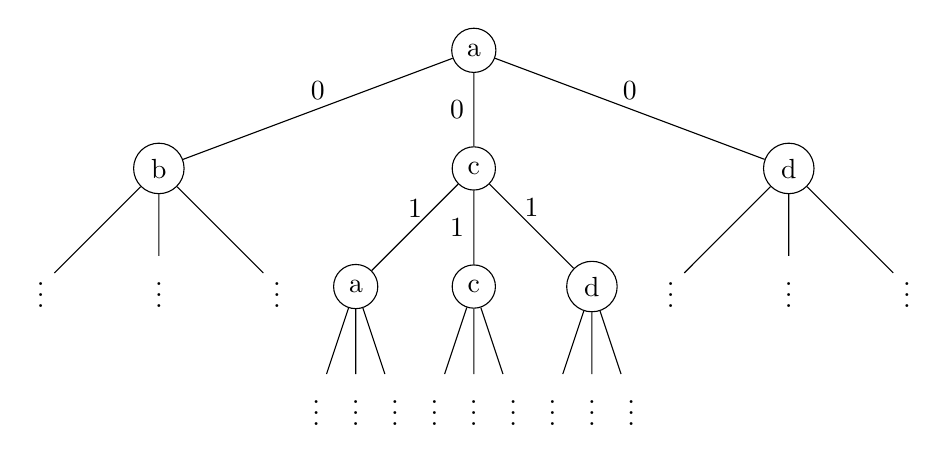
\begin{tikzpicture}
\node [circle,draw] (1){a}
  child {node [circle,draw] (2) {b}
      child {node {$\vdots$}}
      child {node {$\vdots$}}
      child {node {$\vdots$}}
      edge from parent node[above] {0}
  }
  child {node [circle,draw] (3) {c}
      child {node[circle,draw] {a}
	      child {node {$\vdots$}}
	      child {node {$\vdots$}}
    	  child {node {$\vdots$}}
		  edge from parent node[above] {1}    
      }
      child {node[circle,draw] {c}
            child {node {$\vdots$}}
            child {node {$\vdots$}}
            child {node {$\vdots$}}
  		    edge from parent node[left] {1} 
      }  
      child {node[circle,draw] {d}
	      child {node {$\vdots$}}
	      child {node {$\vdots$}}
          child {node {$\vdots$}}
          edge from parent node[above] {1}
      }
      edge from parent node[left] {0}
  }
  child {node [circle,draw] (4) {d}
      child {node {$\vdots$}}
      child {node {$\vdots$}}
      child {node {$\vdots$}}
      edge from parent node[above] {0}
};
\end{tikzpicture}
\end{align*}
Persze a többi állapotból is meg kéne rajzolni a kifutó ágakat, valamint a fa mélységben végtelen, hiszen a program futása sose ér véget, a fa egy tetszőleges gyökérből kiinduló útja jelenti a program egyik lehetséges futását, ezért is hívjuk ezt végrehajtási útnak.

Ebben a modellben tehát nincs valódi párhuzamosság. Az utasítások egymás után hajtódnak végre, de bizonyos megkötések mellett tetszőleges sorrendben. Ezt hívjuk elágazó idejű (v. összefésüléses) szemantikának. Természetesen az absztrakt programot lehet valódi párhuzamos programmal implementálni, de működésének meg kell felelnie az ilyen párhuzamosság nélküli program működésével. A modell szintjén a valódi párhuzamosság kezelhetetlenül bonyolult programokat adna.

Elvárjuk, hogy a fának minden útjára teljesüljön a feltétlenül pártatlan ütemezés. Ez azt jelenti, hogy minden úton minden programhalmazbeli címke végtelen sokszor szerepeljen. Másképp fogalmazva, a futás során minden pillanatban legyen garantálva, hogy az ütemezés még végtelen sokszor kiválaszt minden utasítást. Előfordulhat, hogy egy utasítás csak ritkán fordul elő, míg mások akár egymás után többször is, és az is előfordulhat, hogy egy utasítás valahogy mindig akkor választódik ki, amikor a feltétele hamisra értékelődik ki. A lényeg, hogy néha mindenkinek ki kell választódnia. Elérhető állapotoknak azokat nevezzük, amelyek rajta vannak a fa végrehajtási útjain.
\end{document}
